\documentclass{article}
\usepackage[utf8]{inputenc}

\title{Tarea I Estadiatica II}
\author{Luis Medardo Pavón Pérez }
\date{Marzo 2021}

\usepackage{natbib}
\usepackage{graphicx}
\usepackage{listings}

\usepackage{minted}

\begin{document}

\maketitle

\section{Ejercicio 1}

Sea $Z_t$ un proceso, donde t es un numero par, donde $Z_t$ es una secuencia de variables aleatorias tal que:\\
\\
 $Z_t= \left \{\begin{array}{rl}  1 & \text{si } P[1]=\frac{1}{2} \\   -1 & \text{si }  P[-1]= \frac{1}{2} \end{array} \right. $\\
 
Si t es impar, $Z_t= Z_{t-1}$\\

1) El proceso es estacipnario de orden 1?\\

P.D.\\

$ P[Z_{t1} \leq x] = P[Z_{t2} \leq x]= \dotsc = P[Z_{tn}] \leq x] $ \\

Definimos z:\\

$X_t= 1-2 Z_t$ , as{í} vemos que $X_t ~ B(\frac{1}{2}$\\

Entonces, observamos que:\\

$ X_t= \left \{\begin{array}{rl}  1 & \text{si } P[1]=\frac{1}{2} \\   -1 & \text{si }  P[-1]= \frac{1}{2} \end{array} \right.  \forall t $\\


Entonces \\

$F(X_{t1}) = F(X_{t2})= ... = F(X_{tn})$\\


b) El proceso es estacionario de orden 2?\\

$F(X_{t1},X_{t2}) = F(X_{t2},X_{t3})= \dotsc = F(X_{ti},X_{tj}) = P[Z_{t1} \leq Z, Z_{t2} \leq Z] = P[Z_t \leq z] = 1-F_z(\frac{1-Z}{2})$\\

\section{Ejercicio 2}\\

Sea $Z_t= U\sin(\pi t)+V\cos(2\pi t)$ donde U,V son v.a. con media 0 y varianza 1, U,V.\\

a) $Z_t$ es debilmente estacionario?\\

P.D $E[Z_t]= \mu $ \\

$E[Z_t] = E[U\sin(\pi t)+V\cos(2\pi t)] =E[U\sin(\pi t)]+E[V\cos(2\pi t)] = 0$\\

P.D. $\gamma_Z (t,s) = Cov(Z_t,Z_s) = E[Z_s Z_t]$\\


Donde: $E[Z_s Z_t] = E[(U\sin(\pi t)+V\cos(2\pi t))(E[U\sin(\pi s)+V\cos(2\pi s)])] $\\

$= E[U^2 \sin (\pi t) \sin (\pi s) + V^2 \cos (2\pi t) \cos (2\pi s) = E[U^2] \sin (\pi t) \sin (\pi s)+ E[V^2] \cos (2\pi t) \cos (2\pi s)$\\

$\sin (\pi t) \sin (\pi s) + \cos (2\pi t) \cos (2\pi s) = \frac{1}{2}[\cos (\pi h) - \cos (-\pi h)] = f(h)$\\


\therefore $X_t$ es debilmente estacionario.\\

\section{Ejercicio 3}\\


Probar si los procesos son debilmente estacionarios.\\

a) $Z_t = A \sin(2 \pi t + \theta)$  con  A  constante  . $\theta ~ U(0,2\pi)$\\

$E[Z_t]=E[A \sin(2 \pi t + \theta)] = A \int{0}{2} \sin(2\pi t + \theta) \,d\theta= 0  $  por ser una funcion par. \\


$E[(Z_t)^2]= A^2 \int{0}{2} \sin^2 (2\pi t + \theta) \,d\theta =  A^2 \pi < \infty$ \\


$\gamma _Z (t,s) = Cov (Z_t, Z_s) = E[Z_t, Z_s] - E[Z_t]E[Z_s] = E[Z_t, Z_s] = E[(A \sin(2 \pi t + \theta))(A \sin(2 \pi s + \theta))]$\\


$= A^2 E[(\sin(2 \pi t + \theta))(\sin(2 \pi s + \theta))]=0$\\


\therefore $Z_t$ es debilmente estacionario.\\


b) $Z_t = A \sin(2 \pi t + \theta)$  con  A  una  v.a. con media 0 y var  1.\\


$E[Z_t]=E[A \sin(2 \pi t + \theta)]= E[A] \sin(2 \pi t + \theta)  =  0$\\

$Var(Z_t) = E[Z_t^2]-E[Z_t]^2 = E[Z_t^2] = E[(A \sin(2 \pi t + \theta))^2] = E[A^2] \sin(2 \pi t + \theta)=\sin(2 \pi t + \theta) <\infty $\\

$\gamma_ {Z_t} (t,s) = Cos(Z_t,Z_x)= E[Z_t Z_s]= E[(A \sin(2 \pi t + \theta))(A \sin(2 \pi s + \theta))]= E[A^2] \sin(2 \pi t + \theta)(\sin(2 \pi s + \theta)$\\


$= \sin(2 \pi t + \theta)(\sin(2 \pi s + \theta) = \frac{1}{2} [\cos (2 \pi h)-\cos (2 \pi (-h) +2 \theta] < \infty$\\

$Z_t$ es debilmente estacionario \\


c) $Z_t = (-1)^t A $, A una v.a. con media 0 y varianza 1 \\


$E[Z_t] = E[(-1)^t A] = E[A] E[(-1)^t] =0 $\\


$Var[Z_t] =E[Z_t ^2] -E[Z_t]^2 = E[Z_t ^2] = E[((-1)^t A)^2] = E[((-1)^{t^2} A^2)] = E[((-1)^{2t}] = (-1)^{2t} < \infty $\\


$\gamma_{Z_t} (t,s) = Cov(Z_t,Z_s) = E[Z_t Z_s] - E[Z_t]E[Z_s]= E[Z_t Z_s]=E[((-1)^t A)((-1)^s A)]=E[A^2 (-1)^{t+s}] = E[A^2]E[(-1)^{t+s}]$\\

$ \gamma_{Z_t} = \left \{\begin{array}{rl}  1 & \text{si } t+s es par \\   -1 & \text{si }  t+s es par \end{array} \right.  \forall t $\\


\section{Ejercicio 4}\\

P.D.


$\rho_0 = 1$


Sabemos que $\rho_x = \frac{\gamma_x}{Var(X)}$\\

As{í} mismo ,por definici{ó}n   $\gamma_0 = Var(X)$\\

Entonces:\\

$\rho_0 = \frac{\gamma_0}{Var(x)} =\frac{Var(x)}{Var(x)}=1 $\\

P.D.  $|\rho_k| \leq 1$\\

Sabemos por propiedad que  $|\gamma_k|\leq \gamma_0$\\


Entonces, dividiendo ambos lados entre $\gamma_0$ y como $\gamma_0 = Var(Z_t) \geq 0$ por definici{ó}n, entonces $\gamma_0=|\gamma_0| $\\


As{í}: $\frac{|\gamma_k|}{\gamma_0} \leq \frac{|\gamma_k|}{\gamma_0} \rightarrow |\frac{\gamma_k}{\gamma_0}| \leq \frac{\gamma_0}{\gamma_0}=1 $\\


\rightarrow  $|\rho_k| \leq 1$ \\


P.D.  $\rho_k= \rho_{-k}$\\

Por propiedades de la función de autocovarianza tenemos que: $ \gamma_x = \gamma_{-x}$ \\


As{í},  $\rho_k = \frac{\gamma_x}{var(x)} = \frac{\gamma_{-x}}{var(x)} = \rho_{-x}$\\

\section{Ejercicio 5} \\

\begin{minted}{python}
import pandas as pd
import numpy as np
import matplotlib.pyplot as plt
from matplotlib import pyplot
import seaborn as sns
import warnings
import itertools
warnings.filterwarnings("ignore")
plt.style.use('fivethirtyeight')
import statsmodels.api as sm
from statsmodels.graphics.tsaplots import plot_acf
from statsmodels.graphics.tsaplots import plot_pacf
from statsmodels.tsa.stattools import adfuller
from statsmodels.tsa.ar_model import AR
from statsmodels.tsa.arima_model import ARMA

from math import sqrt
import matplotlib
from random import random


Dada la serie de tiempo:
53,43,66,48,52,42,44,56,44,58,41,54,51,56,38,56,49,52,_
32,52,59,34,57,39,60,40,52,44,65,43

a) Grafica la serie.

b) Calcular $\rho_k$ , para  k=0,1,2,3,4,5

c) Calcular la PACF $\hat{\phi_{k,k}}$ , para k=0,1,2,3,4,5

#a)
X_t=[53,43,66,48,52,42,44,56,44,58,41,54,51,56,38,56,49,52,32,_
52,59,34,57,39,60,40,52,44,65,43]

plt.plot(X_t)
plt.title('Serie de tiempo')
plt.show()
\end{minted}

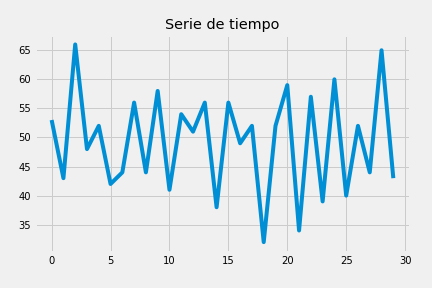
\includegraphics{Serie.png}

\begin{minted}{python}
# b)

X_t_k=pd.DataFrame(X_t,columns=['X'])
X_t_k['Xt-1']=X_t_k['X'].shift(1)
X_t_k['Xt-2']=X_t_k['X'].shift(2)
X_t_k['Xt-3']=X_t_k['X'].shift(3)
X_t_k['Xt-4']=X_t_k['X'].shift(4)
X_t_k['Xt-5']=X_t_k['X'].shift(5)

Covs=X_t_k.cov()
Covs

Rho_1=(Covs['X']['Xt-1'])/ ((X_t_k['X'].std())*(X_t_k['Xt-1'].std()))
Rho_2=(Covs['X']['Xt-2'])/ ((X_t_k['X'].std())*(X_t_k['Xt-2'].std()))
Rho_3=(Covs['X']['Xt-3'])/ ((X_t_k['X'].std())*(X_t_k['Xt-3'].std()))
Rho_4=(Covs['X']['Xt-4'])/ ((X_t_k['X'].std())*(X_t_k['Xt-4'].std()))
Rho_5=(Covs['X']['Xt-5'])/ ((X_t_k['X'].std())*(X_t_k['Xt-5'].std()))
Rho_k=[Rho_1,Rho_2,Rho_3,Rho_4,Rho_5]

#Sigma
sig_1_1=Rho_1
sig_2_2=(Rho_2-sig_1_1*Rho_1)/(1-(sig_1_1*Rho_1))
sig_2_1=sig_1_1-(sig_2_2*sig_1_1)
sig_3_3=(Rho_3-((sig_2_1*Rho_2)+(sig_2_2*Rho_1)))_
/(1-((sig_2_1*Rho_1)+(sig_2_2*Rho_2)))
sig_3_2=sig_2_2-(sig_3_3*sig_2_1)
sig_3_1=sig_2_1-(sig_3_3*sig_2_2)
sig_4_4=(Rho_4-((sig_3_1*Rho_3)+(sig_3_2*Rho_2)+(sig_3_3*Rho_1)))_
/(1-((sig_3_1*Rho_1)+(sig_3_2*Rho_2)+(sig_3_3*Rho_3)))
sig_4_3=sig_3_3-(sig_4_4*sig_3_1)
sig_4_2=sig_3_2-(sig_4_4*sig_3_2)
sig_4_1=sig_3_1-(sig_4_4*sig_3_3)
sig_5_5=(Rho_5-((sig_4_1*Rho_4)+(sig_4_2*Rho_3)+(sig_4_3*Rho_2)+(sig_4_4*Rho_1)))_
/(1-((sig_4_1*Rho_1)+(sig_4_2*Rho_2)+(sig_4_3*Rho_3)+(sig_4_4*Rho_4)))


\end{minted}



\section{Ejercicio 6}\\

Encontrar la ACFP $\rho_k$  y PACF $\theta_{k,k}$  para los siguientes procesos: \\

\subsection{a)}\\
a) \\

$X_t = 0.5 x_{t-1} + W_t$ \\

El proceso $X_t$ es un proceso AR(1) con $ \abs(\theta) <1 $  por lo que  $E[X_t]=0 $

Así mismo, por lo desarrollado en clase, tenemos que:\\

$\gamma_k = \theta^k \gamma_0$   con  $\theta=0.5$  tenemos que  $\gamma_k = (0.5)^k \gamma_0 $\\

As{í}, $\rho_k = (0.5)^k $\\

Por otro lado,

$\theta_{k+1,k+1} = \frac{\rho_{k+1}-[\sum_{j=1}^{k} \theta_{k,j}\rho_{k+1-j} ]}{1- [\sum_{j=1}^{k} \theta_{k,j}\rho_{j} ]}$\\

$\theta_{k+1,j} =\theta_{k,j}-\theta_{k+1,k+1}\theta_{k,k+1-j} $\\

En particular para este caso: \\

$\theta_{1+1,1+1} = \frac{\rho_{2}-\theta_{1,1}\rho_{1} }{1-\theta_{1,1}\rho_{1}} = \frac{(0.5)^2 -(0.5)(0.5)}{1-(0.5)(0.5)} =0 $\\

$\theta_{2+1,2+1} = \frac{\rho_{3}-[\sum_{j=1}^{2} \theta_{2,j}\rho_{3-j} ]}{1- [\sum_{j=1}^{2} \theta_{2,j}\rho_{j}]} = \frac{(0.5)^3 -(0.5)(0.5)^2 - 0(0.5)^2}{1-(0.5)(0.5)-0(0.5)} = 0 $  \\

Entonces concluimos que $\theta_{k,k} = 0$ si $k12$

\subsection{b)}

b) 
$X_t = 0.5 x_{t-1} + W_t$ \\

Análogamente al ejercicio a, tenemos que $E[X_t]=0  y \rho_k = (0.98)^k$ \\

Así mismo, bandonos en el ejercicio anterior, se concluye que: \\

$\theta_{k,k} = \left\{\begin{array}{rl}  1 & \text{si } k =0 \\   0.98 & \text{si } k =1 \\  0 & \text{si}  K>1 \end{array} \right. $\\

\subsection{c)}

c)$X_t = 1.3 x_{t-1} - 0.4 x_{t-2} + W_t$ \\

Por lo visto en clase concluimos que $X_t $ es un proceso AR(2), por lo que tenemos que:\\

$\rho_1 = \frac{\theta_1}{1-\theta_2}    ;   \rho_2 = \frac{\theta_1 ^2 + \theta_2(1-\theta_2)}{1-\theta_2}$\\

Así en general:\\

$\rho_k = \theta_1 \rho_{k-1} + \theta_2 \rho_{k-2} $\\

con $\theta_1 = 1.3  y \theta_2= -0.4 $ tenemos: \\

$\rho_1 = \frac{1.3}{1+.4} = \frac{1.3}{1.4}    ;   \rho_2 = \frac{(1.3) ^2 - (0.4)(1+0.4)}{1+0.4} = = \frac{(1.3) ^2 - (0.4)(1.4)}{1.4}$\\

$\rho_3 = (1.3)(\frac{(1.3) ^2 - (0.4)(1.4)}{1.4}) - (0.4) \frac{1.3}{1.4} $\\

$\rho_4 = (1.3)(\frac{(1.3) ^3 - (0.4)(1.4)(1.3)- (0.4)(1.3)}{1.4}) - (0.4) (\frac{(1.3)^2 -  (0.4)(1.4)}{1.4} )$\\

$\rho_5 = (1.3)(\frac{(1.3) ^4 - (0.4)(1.4)(1.3)^2- (0.4)(1.3)+ (0.4)^2(1.4)^2}{1.4}) - (0.4) (\frac{(1.3)^3 -  (0.4)(1.4)(1.3)-(0.4)(1.3)}{1.4} )$\\

Ahora, para $\theta_{k,k}$ tenemos: \\

$\theta_{1,1} = \rho_1 = \frac{1.3}{1.4}$

$\theta_{1+1,1+1} = \frac{\rho_{2}-\theta_{1,1}\rho_{1} }{1-\theta_{1,1}\rho_{1}} = \theta_2 = -0.4 $\\

$\theta_{1+1,1} = =\theta_{1,1}-\theta_{2,2}\theta_{1,1}= \frac{\theta_1}{1-\theta_2} -\theta_2 \frac{\theta_1}{1-\theta_2} =\theta_1 $

$\theta_{2+1,2+1} = \frac{\rho_{3}-[\sum_{j=1}^{2} \theta_{2,j}\rho_{3-j} ]}{1- [\sum_{j=1}^{2} \theta_{2,j}\rho_{j} ]} = \frac{\rho_{3}-\theta_{2,1}\rho_{2} -\theta_{2,2}\rho_{1}}{1-\theta_{2,1}\rho_{1} -\theta_{2,2}\rho_{2} } $\\

$\theta_{2+1,2+1} = \frac{\theta_1 \rho_2 + \theta_2 \rho_1 - \theta_1 \rho_2 - \theta_2 \rho_1}{1-\theta_{2,1}\rho_{1} -\theta_{2,2}\rho_{2}}  = 0 $\\

Entonces:\\ 


$\theta_{k,k} = \left\{\begin{array}{rl}  \frac{\theta_1}{1-\theta_2} & \text{si } k =1 \\  \theta_2 & \text{si } k =2 \\  0  & \text{si}  K>2 \end{array} \right. $\\

Para este caso, con $\theta_1 =1.3 ,   \theta_2 = -0.4 $

$\theta_{k,k} = \left\{\begin{array}{rl}  \frac{1.3}{1.4} & \text{si } k =1 \\  -0.4 & \text{si } k =2 \\  0  & \text{si}  K>2 \end{array} \right. $\\

\subsection{d)}

d)$X_t = 1.2 x_{t-1} - 0.8 x_{t-2} + W_t$ \\

An{á}logamente, tenemos:\\

$\rho_1 = \frac{1.2}{1+.8} = \frac{1.2}{1.8}    ;   \rho_2 = \frac{(1.2) ^2 - (0.8)(1+0.8)}{1+0.8} = = \frac{(1.2) ^2 - (0.8)(1.8)}{1.8}$\\

$\rho_3 = (1.2)(\frac{(1.2) ^2 - (0.8)(1.8)}{1.8}) - (0.8) \frac{1.2}{1.8} $\\

$\rho_4 = (1.2)(\frac{(1.2) ^3 - (0.8)(1.8)(1.2)- (0.8)(1.2)}{1.8}) - (0.8) (\frac{(1.2)^2 -  (0.8)(1.8)}{1.8} )$\\

$\rho_5 = (1.2)(\frac{(1.2) ^4 - (0.8)(1.8)(1.2)^2- (0.8)(1.2)+ (0.8)^2(1.8)^2}{1.8}) - (0.8) (\frac{(1.2)^3 -  (0.8)(1.8)(1.2)-(0.8)(1.2)}{1.8} )$\\

Adem{á}s :\\

$\theta_{k,k} = \left\{\begin{array}{rl}  \frac{1.2}{1.8} & \text{si } k =1 \\  -0.8 & \text{si } k =2 \\  0  & \text{si}  k>2 \end{array} \right. $\\

\section{Ejercicio 7}\\

Encontrar el rango de valores que puede tomar $\alpha$ tal que el preceso $X_t$ sea estacionario.\\

$ X_t = X_{t-1} + \alpha X_{t-2} + w_t$\\

Tenemos el polinomio: \\

$W_t = (1-B - \alpha B^2) X_t$\\

Para que el proceso sea estacionario, se necesita cumplir que,  $ B >|1|$  , entonces: \\

$B= \frac{-1 \pm \sqrt{(-1)^2 - 4 (-\alpha)(1)}}{2(-\alpha)}$\\

As{í} buscamos $\alpha $ tal que:\\

$\frac{-1 \pm \sqrt{(-1)^2 - 4 (-\alpha)(1)}}{2(-\alpha)} > |1|$ \\

Entonces: \\

$\frac{-1 + \sqrt{(-1)^2 - 4 (-\alpha)(1)}}{2(-\alpha)} > |1|$ \\

$\frac{-1 + \sqrt{(-1)^2 - 4 (-\alpha)(1)}}{2(-\alpha)} > 1$   y  $\frac{-1 + \sqrt{(-1)^2 - 4 (-\alpha)(1)}}{2(-\alpha)} < -1$  \\

Primero:\\

$\frac{-1 + \sqrt{(-1)^2 - 4 (-\alpha)(1)}}{2(-\alpha)} > 1 \rightarrow -1 + \sqrt{(-1)^2 - 4 (-\alpha)(1)} < 2(-\alpha)  \rightarrow \sqrt{(-1)^2 - 4 (-\alpha)(1)} < 2(-\alpha)+1 $\\
$\rightarrow  1 + 4(\alpha) < 4(\alpha)^2-2\alpha +1  \rightarrow  4(\alpha) < 4(\alpha)^2-2\alpha  \rightarrow  0 < 4(\alpha)^2-6\alpha = 2\alpha(2\alpha-3)  $\\

$\rightarrow  2\alpha >0$ y $2\alpha-3 >0  \rightarrow  \alpha >0 y \alpha > \frac{3}{2}$\\

Por otro lado: \\

$\frac{-1 + \sqrt{(-1)^2 - 4 (-\alpha)(1)}}{2(-\alpha)} < -1  \rightarrow  -1 + \sqrt{(-1)^2 + 4 (\alpha)}> 2\alpha  \rightarrow  \sqrt{1 + 4 (\alpha)}> 2\alpha +1 $\\

$\rightarrow  1 + 4 (\alpha)> 4\alpha^2 +2\alpha +1  \rightarrow  4 (\alpha)> 4\alpha^2 +2\alpha \rightarrow 0 > 4\alpha^2 -2\alpha = 2\alpha (2\alpha -1) $\\

$ \alpha >0 $  y  $(2\alpha -1) > 0  \rightarrow  \alpha > \frac{1}{2}$\\

Para la otra raiz, tenemos:\\

$\frac{-1 - \sqrt{(-1)^2 - 4 (-\alpha)(1)}}{2(-\alpha)} > |1|$ \\

$\frac{-1 - \sqrt{(-1)^2 - 4 (-\alpha)(1)}}{2(-\alpha)} > 1$   y  $\frac{-1 - \sqrt{(-1)^2 - 4 (-\alpha)(1)}}{2(-\alpha)} < -1$  \\

Primero:\\

$\frac{-1 - \sqrt{(-1)^2 - 4 (-\alpha)(1)}}{2(-\alpha)} > 1 \rightarrow -1 - \sqrt{1 + 4 (\alpha)} < 2(-\alpha)  \rightarrow \sqrt{1 + 4 (\alpha)} > -1-2(\alpha)  \rightarrow  1 + 4 (\alpha) > 1-4(\alpha) +4(\alpha)^2  \rightarrow  0 > -8(\alpha) +4(\alpha)^2 =4(\alpha)(-2 +\alpha)  $\\

$\rightarrow 4(\alpha)(-2 +\alpha) > 0  \rightarrow  \alpha >0 $ y $ \alpha >2 $\\

Por otro lado: \\

$\frac{-1 - \sqrt{1 + 4 (\alpha)}}{2(-\alpha)} < -1  \rightarrow  -1 - \sqrt{1 + 4 (\alpha)}> 2\alpha  -\sqrt{1 + 4 (\alpha)}> 2\alpha +1 $\\

$\sqrt{1 + 4 (\alpha)} < 2\alpha +1 \rightarrow 1 + 4 (\alpha) < 4\alpha^2 +2\alpha +1  \rightarrow  0 < 4\alpha^2 -2\alpha=  2\alpha(2\alpha-1)  $\\

$2\alpha(2\alpha-1)> 0 \rightarrow  2\alpha >0 $ y $\alpha > \frac{1}{2}$\\

Entonces:

$\alpha \in (\frac{2}{3}, \infty) \cap (2,\infty)  \rightarrow \alpha \in (2,\infty) $\\

Suponiendo $\alpha = \frac{-1}{2}$ calcula la ACF\\

Por lo visto en clase concluimos que $X_t $ es un proceso AR(2), por lo que tenemos que:\\

$\rho_1 = \frac{\theta_1}{1-\theta_2}    ;   \rho_2 = \frac{\theta_1 ^2 + \theta_2(1-\theta_2)}{1-\theta_2}$\\

Así en general:\\

$\rho_k = \theta_1 \rho_{k-1} + \theta_2 \rho_{k-2} $\\

con $\theta_1 = 2  y \theta_2= -0.5 $ tenemos: \\

$\rho_1 = \frac{1}{1.5}    ;   \rho_2 = \frac{1 -0.5(1.5)}{1.5}$\\

Así en general:\\

$\rho_k = \rho_{k-1} -(0.5) \rho_{k-2} $\\


\section{Ejercicio 8}\\

Sea $X_t = W_t + 1.2 W_{t-1} + 0.5 W_{t-2}$  encuentra una expresi{ó}n para la ACF y la PACF

\subsection{ACF}\\

$E[x_t] = E[W_t + 1.2 W_{t-1} + 0.5 W_{t-2}] = E[W_t] + 1.2 E[W_{t-1}] + 0.5 E[W_{t-2}] = 0$\\

$\gamma_k = E[X_t X_{t+k}]$\\

si $k=0$ entonces: \\

$\gamma_k = \gamma_0 = E[X_t X_t] = E[X_t^2]=E[(W_t + 1.2 W_{t-1} + 0.5 W_{t-2})^2] = E[W_t ^2 +2(1.2)W_t W_{t-1} + 2(0.5) W_t W_{t-2} + 2(1.5)(0.5)W_{t-1} W_{t-2} +(1.2)^2 W_{t-1}^2+ (0.5)^2 W_{t-2}^2] =  E[W_t ^2] + E[2(1.2)W_t W_{t-1} ]+E[ 2(0.5) W_t W_{t-2}] + E[2(1.5)(0.5)W_{t-1} W_{t-2}] +E[(1.2)^2 W_{t-1}^2]+E[ (0.5)^2 W_{t-2}^2] =E[W_t ^2] + E[(1.2)^2 W_{t-1}^2]+E[ (0.5)^2 W_{t-2}^2] = E[W_t ^2] +(1.2)^2 E[ W_{t-1}^2]+(0.5)^2 E[W_{t-2}^2] = 1+(1.2)^2 +(0.5)^2  $\\

Si $k =1 $ \\

$\gamma_k = E[X_t X_{t-1}] = E([W_t + 1.2 W_{t-1} + 0.5 W_{t-2})(W_{t-1} + 1.2 W_{t-2} + 0.5 W_{t-3})]= (1.2)E[W_{t-1}^2] + (0.5)(1.2)E[W_{t-2}^2] = 1.2+(1.2)(0.5)=1.2(1.5)$\\

Si $k =2 $ \\

$\gamma_k = E[X_t X_{t-2}] = E([W_t + 1.2 W_{t-1} + 0.5 W_{t-2})(W_{t-2} + 1.2 W_{t-3} + 0.5 W_{t-4})]= (0.5)E[W_{t-2}^2] = (0.5) $\\

Si $k> 2,  \gamma_k =0 $\\

Como $\rho_k = \frac{\gamma_k}{\gamma_0}  entonces, $\\

$\rho_{k} = \left\{\begin{array}{rl}  1 & \text{si } k =0  \\ \frac{1.2(1.5)}{1+(1.2)^2+(0.5)^2} & \text{si } k =1 \\  \frac{0.5}{1+(1.2)^2+(0.5)^2} & \text{si } k =2 \\  0  & \text{si}  K>2 \end{array} \right. $\\

\subsection{PACF}\\

Recordando, tenemos: \\

$\theta_{k+1,k+1} = \frac{\rho_{k+1}-[\sum_{j=1}^{k} \theta_{k,j}\rho_{k+1-j} ]}{1- [\sum_{j=1}^{k} \theta_{k,j}\rho_{j} ]}$\\

Entonces: \\

$\gamma_{1,1} = \rho_1 = \frac{1.2(1.5)}{1+(1.2)^2+(0.5)^2} $

$\theta_{1+1,1+1} = \frac{\rho_{2}-\theta_{1,1}\rho_{1} }{1-\theta_{1,1}\rho_{1}} = \frac{\rho_{2} -  \rho_{1}^2}{1-\rho_{1}^2} = \frac{(\frac{0.5}{1+(1.2)^2+(0.5)^2})-(\frac{1.2(1.5)}{1+(1.2)^2+(0.5)^2})^2}{1-(\frac{(1.2)(1.5)}{1+(1.2)^2+(0.5)^2})^2} $\\

\section{Ejercicio 9}\\

Demuestra si el proceso $X_t$ es estacionario.

$X_t = W_t + 0.1W_{t-1} +0.21W_{t-2} $\\

$E[X_t] = 0 $\\

$\gamma_k = E[X_t X_{t-k}$ \\

Para $k=0$\\

$\gamma_0 = Var(X_t)= E[(W_t + 0.1W_{t-1} +0.21W_{t-2})(W_t + 0.1W_{t-1} +0.21W_{t-2})] = E[W_t^2]+(0.1)^2E[W_{t-1}^2]+(0.21)^2E[W_{t-2}^2] = 1 + +(0.1)^2+(0.21)^2$\\

Para $K=1$ \\

$\gamma_1 = E[X_t X_{t-1}] = E[(W_t + 0.1W_{t-1} +0.21W_{t-2})(W_{t-1} + 0.1W_{t-2} +0.21W_{t-3})] = (0.1)E[W_{t-1}^2]+(0.21)(0.1)E[W_{t-2}^2] = (0.1)+(0.21)(0.1) $\\

Para $K=2$ \\

$\gamma_2 = E[X_t X_{t-2}] = E[(W_t + 0.1W_{t-1} +0.21W_{t-2})(W_{t-2} + 0.1W_{t-3} +0.21W_{t-4})] = (0.21)(0.1)E[W_{t-2} ^2] =(0.21)(0.1)$  \\

Para $k>2$ \\

$ \gamma_k = 0 $\\

As{í} tenemos:\\

$\gamma_{k} = \left\{\begin{array}{rl}  1 + +(0.1)^2+(0.21)^2 & \text{si } k =0  \\ (0.1)+(0.21)(0.1) & \text{si} k =1 \\  (0.21)(0.1) & \text{si } k =2 \\  0  & \text{si}  K>2 \end{array} \right. $\\

$\rho_{k} = \left\{\begin{array}{rl}  1 & \text{si } k =0  \\ \frac{(0.1)+(0.21)(0.1)}{1+(0.1)^2+(0.21)^2} & \text{si } k =1 \\  \frac{(0.21)(0.1)}{1+(0.1)^2+(0.21)^2} & \text{si } k =2 \\  0  & \text{si}  K>2 \end{array} \right. $\\


As{í}:\\
$\theta_{1+1,1+1} = \frac{\rho_{2}-\theta_{1,1}\rho_{1} }{1-\theta_{1,1}\rho_{1}} = \frac{\rho_{2} -  \rho_{1}^2}{1-\rho_{1}^2} = \frac{(\frac{(0.1)(0.21)}{1+(0.1)^2+(0.21)^2})-(\frac{(0.1)(1.21)}{1+(0.1)^2+(0.21)^2})^2}{1-(\frac{(1.21)(0.1)}{1+(0.1)^2+(0.21)^2})^2} $\\

\section{Ejercicio 10}\\

De los modelos siguientes, simluar 1000 observaciones, calcular la ACF y PACF para k=0,1,2,...,10 y estimarlas a partir de las simulaciones.\\

\begin{minted}{python}

#A
W=np.random.randn(1000)
X_t_1=np.zeros(1000)

for t in range(1,len(W)):
    X_t_1[t]=(0.5)*X_t_1[t-1]+W[t]

\end{minted} 

Estimaci{ó}n gr{á}fica de la ACF y PACF usando las simulaciones:

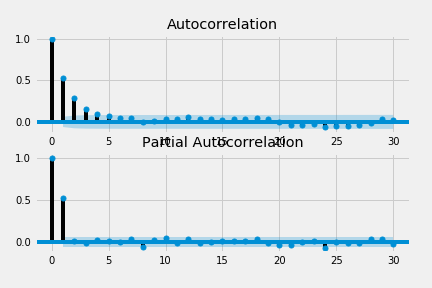
\includegraphics{ACF_PACF_1.png}

\begin{minted}{python}
#B  
W=np.random.randn(1000)
X_t_2=np.zeros(1001)

for t in range(2,len(W)):
    X_t_2[t]=(0.25)*X_t_1[t-1]+(0.3)*X_t_1[t-2]+W[t]
\end{minted}    


Estimaci{ó}n gr{á}fica de la ACF y PACF usando las simulaciones:

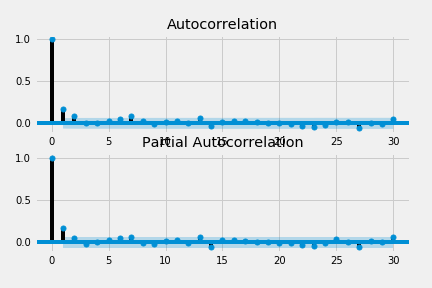
\includegraphics{ACF_PACF_2.png}


\begin{minted}{python}
#C
W=np.random.randn(1000)
X_t_3=np.zeros(1001)

for t in range(1,len(W)):
    X_t_3=(0.13)*W[t-1]+W[t]
\end{minted}    


Estimaci{ó}n gr{á}fica de la ACF y PACF usando las simulaciones:

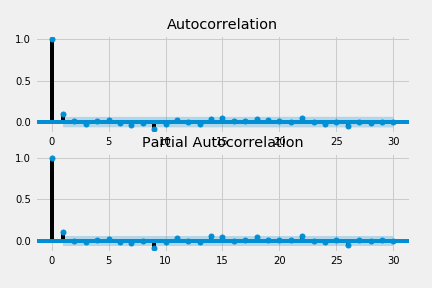
\includegraphics{ACF_PACF_3.png}

\begin{minted}{python}    
#D
W=np.random.randn(1000)
X_t_4=np.zeros(1001)

for t in range(2,len(W)):
    X_t_4=(0.23)*W[t-1]+(0.3)*W[t-2]+W[t]

\end{minted}


Estimaci{ó}n gr{á}fica de la ACF y PACF usando las simulaciones:

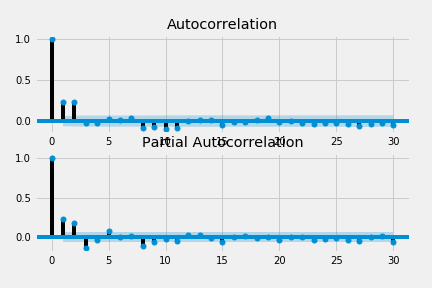
\includegraphics{ACF_PACF_4.png}

\end{document}
